%%% Econ712: Macroeconomics I
%%% Fall 2020
%%% Danny Edgel
%%%
% Due on Canvas Thursday October 22, 11:59pm Central Time
%%%

%%%
%							PREAMBLE
%%%

\documentclass{article}

%%% declare packages
\usepackage{amsmath}
\usepackage{amssymb}
\usepackage{array}
\usepackage{bm}
\usepackage{changepage}
\usepackage{centernot}
\usepackage{graphicx}
\usepackage[shortlabels]{enumitem}
\usepackage{fancyhdr}
	\fancyhf{} % sets both header and footer to nothing
	\renewcommand{\headrulewidth}{0pt}
    \rfoot{Edgel, \thepage}
    \pagestyle{fancy}
	
%%% define shortcuts for set notation
\newcommand{\N}{\mathbb{N}}
\newcommand{\Z}{\mathbb{Z}}
\newcommand{\R}{\mathbb{R}}
\newcommand{\Q}{\mathbb{Q}}
\newcommand{\lmt}{\underset{x\rightarrow\infty}{\text{lim }}}
\newcommand{\neglmt}{\underset{x\rightarrow-\infty}{\text{lim }}}
\newcommand{\zerolmt}{\underset{x\rightarrow 0}{\text{lim }}}
\newcommand{\loge}[1]{\text{ln}\left(#1\right)}
\newcommand{\usmax}[1]{\underset{#1}{\text{max }}}
\newcommand{\Mt}{M_{t+1}^t}
\newcommand{\olp}{\overline{p}}
\renewcommand{\L}{\mathcal{L}}
\newcommand{\olq}{\overline{q}}

%%% define column vector command (from Michael Nattinger)
\newcount\colveccount
\newcommand*\colvec[1]{
        \global\colveccount#1
        \begin{pmatrix}
        \colvecnext
}
\def\colvecnext#1{
        #1
        \global\advance\colveccount-1
        \ifnum\colveccount>0
                \\
                \expandafter\colvecnext
        \else
                \end{pmatrix}
        \fi
}

%%% define function for drawing matrix augmentation lines
\newcommand\aug{\fboxsep=-\fboxrule\!\!\!\fbox{\strut}\!\!\!}

\makeatletter
\let\amsmath@bigm\bigm

\renewcommand{\bigm}[1]{%
  \ifcsname fenced@\string#1\endcsname
    \expandafter\@firstoftwo
  \else
    \expandafter\@secondoftwo
  \fi
  {\expandafter\amsmath@bigm\csname fenced@\string#1\endcsname}%
  {\amsmath@bigm#1}%
}


%________________________________________________________________%

\begin{document}

\title{	Problem Set \#7 }
\author{ 	Danny Edgel 					\\ 
			Econ 712: Macroeconomics I		\\
			Fall 2020						\\
		}
\maketitle\thispagestyle{empty}

%%%________________________________________________________________%%%

\noindent\textit{Collaborated with Sarah Bass, Emily Case, Michael Nattinger, and Alex Von Hafften}
\medskip \\

%%%________________________________________________________________%%%

\noindent Consider a two-period overlapping generations model where agents earn $y$ when young and $0$ when old. Housing supply is fixed at $H^s=1$ and preferences are given by 
\[
	U(c_t^t,h_t,c_{t+1}^t) = \loge{c_t^t} + \alpha h_t + \beta c_{t+1}^t 
\]
Assume that the initial old hold the housing stock and $1+\alpha > \beta y$.
\begin{enumerate}
	\item The social planner's problem (SPP) is:
		\[
			\usmax{\{c_t^t,h_t,c^{-t}_t\}^\infty_{t=1}}\loge{c_t^t} + \alpha h_t + \beta c^{t-1}_t \text{ s.t. } h_t=1\text{, }x_t^t+c_t^{t-1}=y
		\]
		The using the budget constraint to solve for the consumption of the old generation as a function of the consumption of the young generation and setting $h_t=1$ in each period, the SPP can be re-written as:
		\[
			\usmax{\{c_t^t\}^\infty_{t=1}}\loge{c_t^t} + \alpha + \beta (y-c_t^t)
		\]
		Where the FOC for $c_t^t$ can be used to solve for the social planner's allocation in each period:
		\begin{align*}
			\frac{1}{x_t^t}-\beta &= 0	\\
			c_t^t &= \frac{1}{\beta}	\\
			c_t^{t-1} &= y-\frac{1}{\beta}	\\
			b_t &= 1
		\end{align*}
		
	\pagebreak	
	\item Let $p_t$ be the price of a house in period $t$.
		\begin{enumerate}[(a)]
			\item The young agent's problem is 
				\[
					\usmax{\{c_t^t,h_t,c_{t+1}^t\}^\infty_{t=1}}\loge{c_t^t} + \alpha h_t + \beta c_{t+1}^t \text{ s.t. } c_t^t + p_th_t = y\text{, }c_{t+1}^t = p_{t+1}h_t
				\]
				
			\item The market clearing conditions are:
				\begin{align*}
					c_t^t + c_t^{t-1} 	&= y &\text{(Goods market)} 	\\
								h_t 	&= 1 &\text{(Housing market)} 
				\end{align*}
			
			\item A competitive general equilibrium is an allocation, $\{c_t^t,h_t,c_t^{t-1}\}_{t=1}^\infty$ and set of prices, $\{p_t\}_{t=1}^\infty$ that solve every agent's problem in each period and allow markets to clear.
			
			\item Using each period's budget constraint, the young agent's problem can be rewritten as a choice of only housing:
				\[
					\usmax{\{h_t\}^\infty_{t=1}}\loge{y-p_th_t} + \alpha h_t + \beta p_{t+1}h_t
				\]
				Using the FOC for housing, we can solve for the agent's optimal housing and consumption rules:
				\begin{align*}
					\frac{p_t}{y-p_th_t} + \alpha + \beta p_{t+1} &= 0				\\
					(y-p_th_t)(\alpha + \beta p_{t+1}) &= p_t 						\\
					p_th_t &= y-\frac{p_t}{\alpha + \beta p_{t+1}}					\\
					h_t		&= \frac{y}{p_t} - \frac{1}{\alpha + \beta p_{t+1}} 	\\
					c_t^t &= y-p_t\left(\frac{y}{p_t} - \frac{1}{\alpha + \beta p_{t+1}}\right) \\
						&= y - y + \frac{p_t}{\alpha + \beta p_{t+1}} = \frac{p_t}{\alpha + \beta p_{t+1}} \\
					c_{t+1}^t &= p_{t+1}\left(\frac{y}{p_t} - \frac{1}{\alpha + \beta p_{t+1}}\right) \\
						&= \frac{p_{t+1}}{p_t} y - \frac{p_{t+1}}{\alpha + \beta p_{t+1}}	\\
						&=  \frac{p_{t+1}}{p_t} \left( y - \frac{p_t}{\alpha + \beta p_{t+1}} \right)
				\end{align*}
				Thus, the optimal rules for each variable and their associated non-negativity conditions are (assuming prices are weakly positive):\footnote{As housing cannot go negative and positively relates to utility, this is a reasonable assumption.}
				\begin{align*}
					h_t		&= \frac{y}{p_t} - \frac{1}{\alpha + \beta p_{t+1}}, &y>\frac{p_t}{\alpha + \beta p_{t+1}} 	\\
					c_t^t &= \frac{p_t}{\alpha + \beta p_{t+1}}, &\alpha>-\beta p_{t+1} \\
					c_{t+1}^t &=  \frac{p_{t+1}}{p_t} \left( y - \frac{p_t}{\alpha + \beta p_{t+1}} \right), &y>\frac{p_t}{\alpha + \beta p_{t+1}}
				\end{align*}
				
			\item In equilibrium, $h_t=1$, so we can solve:
				\begin{align*}
					h_t		&= 1	\\
					\frac{y}{p_t} - \frac{1}{\alpha + \beta p_{t+1}} &= 1 	\\
					\frac{1}{\alpha + \beta p_{t+1}} &= \frac{y}{p_t} - 1  	\\
					\alpha + \beta p_{t+1} &= \frac{1}{\frac{y}{p_t} - 1}	\\
					p_{t+1} &= \frac{p_t}{\beta(y-p_t)} - \frac{\alpha}{\beta}
				\end{align*}
				\begin{center}
					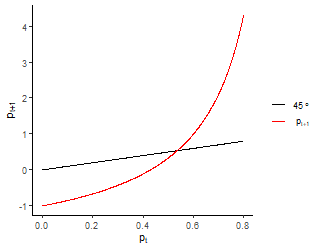
\includegraphics{priceplot.png}
				\end{center}
				
			\item In the steady state, $p_t = p_{t+1}=\overline{p}$ $\forall t$. So, using the law of motion from 2(e):
				\begin{align*}
					\olp &= \frac{\olp}{\beta(y-\olp)} - \frac{\alpha}{\beta}	\\
					\beta\olp + \alpha &= \frac{\olp}{y-\olp}	\\
					(y-\olp)(\beta\olp) + \alpha &= \olp	\\
					y\beta\olp + \alpha y - \beta\olp^2-\alpha\olp - \olp &= 0	\\
					\beta\olp^2 + (\alpha-y\beta + 1)\olp - \alpha y &= 0		\\
					\olp &= \frac{-\alpha+y\beta - 1 \pm\sqrt{(\alpha-y\beta + 1)^2-4\beta\alpha y}}{2\beta}
				\end{align*}
				Since $p$ cannot be negative, the unique, steady-state value of $p$ is
				\[
					\olp = \frac{-\alpha+y\beta - 1 +\sqrt{(\alpha-y\beta + 1)^2-4\beta\alpha y}}{2\beta}
				\]
				
			\item Given the steady-state price of housing and optimal choice of consumption and housing, the competitive allocation is
				\begin{align*}
					h_t		&= \frac{y}{\frac{-\alpha+y\beta - 1 +\sqrt{(\alpha-y\beta + 1)^2-4\beta\alpha y}}{2\beta}} - \frac{1}{\alpha + \beta p_{t+1}}	\\
					c_t^t &= \left(\frac{-\alpha+y\beta - 1 +\sqrt{(\alpha-y\beta + 1)^2-4\beta\alpha y}}{2\beta}\right)	\\
									&\left(\alpha + \left(\frac{-\alpha+y\beta - 1 +\sqrt{(\alpha-y\beta + 1)^2-4\beta\alpha y}}{2\beta}\right)\right)^{-1} \\
					c_{t+1}^t &=  y - \left(\frac{-\alpha+y\beta - 1 +\sqrt{(\alpha-y\beta + 1)^2-4\beta\alpha y}}{2\beta}\right)	\\
									&\left(\alpha + \left(\frac{-\alpha+y\beta - 1 +\sqrt{(\alpha-y\beta + 1)^2-4\beta\alpha y}}{2\beta}\right)\right)^{-1}
				\end{align*}
				Which clearly does not simplify to the social planner's allocation.
		\end{enumerate}

\end{enumerate}


%%%________________________________________________________________%%%


\end{document}












